\newpage
\section{Árboles de Regresión y Clasificación}
\noindent Sea un vector aleatorio $\textbf{x}$ con $p$ los datos de entrada, e $Y$ la variable respuesta. Supóngase también que se toman $n$ observaciones obteniéndose parejas $(\textbf{x}_i,y_i)$. De esta manera, tenemos que las $\textbf{x}_i\in \mathbb{R}^p$.\\
Los métodos de árboles intentan dividir el espacio $\mathbb{R}^p$ y luego en cada región del espacio se ajusta un modelo más simple, incluso una constante.\\
La ventaja de este tipo de métodos es que son fácilmente interpretables, ya que aunque no sea fácil representar el espacio $\mathbb{R}^p$, permiten ser representados como un diagrama de árbol.\\ 
Las  siguientes imágenes procedentes de \textit{Hastie et. al.}\cite{Hastie 2001} muestran el diagrama resultante tras dividir el espacio de observaciones mediante un árbol, 

\begin{figure}[h]
 \centering
  \subfloat[División de $\mathbb{R}^p$]{
   \label{f:división}
    \includegraphics[width=0.4\textwidth]{Documentos Extra/Imagenes/Regiones árboles.png}}
  \subfloat[Diagrama resultante]{
   \label{f:diagrama arbol}
    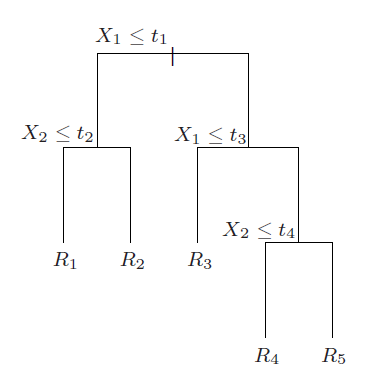
\includegraphics[width=0.4\textwidth]{Documentos Extra/Imagenes/Diagrama de arbol.png}}
 \caption{Representación de la división de $\mathbb{R}^p$ y el diagrama de árbol resultante}
 \label{f:MARC1}
\end{figure}

\noindent Ahora se desarrolla la teoría en profundidad y el algoritmo de los árboles de regresión y de calsificación para luego establecer el algoritmo \textit{random forest}.
\subsection{Árboles de Regresión}
\noindent Sea un vector aleatorio $\textbf{x}$ de variables predictoras como antes y una variable $Y$ de respuesta. 
Supóngase que queremos dividir el espacio de observaciones en $M$ regiones, $R_1,\ldots R_M$, se puede modelar en cada una de las regiones como la constante $c_m$. Por tanto teniendo en cuenta, la siguiente definición. 
\begin{equation}
I_m(\textbf{x})=
\begin{cases}
0\quad& \text{si } x\notin R_m\\
1\quad& \text{si } x\in R_m\\
\end{cases}
\end{equation}
Es decir, la función $I_m(\textbf{x})$ es la función característica de la región $R_m$, por tanto puede construirse el siguiente predictor:
\begin{equation}
f(\textbf{x})=\sum_{m=1}^M c_m I_m(\textbf{x})
\end{equation}

\noindent Si se toma como criterio de ajuste los mínimos cuadrados obtendremos que $\hat{c}_m=ave(y_i|x_i\in R_m)$, ya que es la media condicional de la y sabiendo el valor de x. 

\noindent Para obtener las regiones tenemos que tomar una variable $X_j$ y un valor de separación $s$, es decir, cada separación se puede identificar con una pareja $(j,s)$. 
Por ejemplo, supóngase una separación $(j,s)$ entonces se generan dos regiones del espacio de las observaciones $R_1, R_2$. 
\begin{equation}
R_1=\lbrace\textbf{x}|X_j\leq s\rbrace\quad R_2=\lbrace\textbf{x}|X_j > s\rbrace 
\end{equation}

\noindent Hay que establecer un criterio para elegir que separaciones se deben hacer en particular, para ello se utilizan los mínimos cuadrados:
\begin{equation}
\min_{j,s}\left[\min_{c_1}\sum_{x_i\in R_1}(y_i-c_1)^2+\min_{c_2}\sum_{x_i\in R_2}(y_i-c_2)^2\right]
\end{equation}

\noindent Para optimizar los parámetros $c_1,c_2$ que como se señaló anteriormente se puede utilizar las medias conociendo el valor de $\textbf{x}$. 

\noindent Es posible entonces hacer una algoritmo que busque entre todas

 
\subsection{Árboles de Clasificación }